\documentclass[minted]{protocol}
% Required
\title{Komponentenbasierte Programmierung}
\author{Marc Rousavy}
% Optional
\mysubtitle{Laborprotokoll}
\mysubject{Systemtechnik Labor}
\mycourse{4AHIT 2017/18}
% Version
\myteacher{Michael Borko}
\myversion{1.1}
\mybegin{12. April 2018}
\myfinish{20. April 2018}
% \setcode{frame=single} 			% Add a frame to codes (single, lines)
% \setcode{bgcolor=MyLightGray}		% Add a background to codes (minted only)
% \usemintedstyle{rainbow_dash} 	% autumn, rainbow_dash, tango (default), trac
\begin{document}
% \thispagestyle{fancy}				% Makes the first page fancy too
% \begin{abstract}\end{abstract} 	% Add a short overview
%!TEX root=../protocol.tex	% Optional

\section{Einf{\"u}hrung}

Diese {\"U}bung zeigt die Anwendung von komponentenbasierter Programmierung mittels Webframeworks.

\subsection{Ziele}

Das Ziel dieser {\"U}bung ist die automatisierte Persistierung und Verwendung von Objekten eines vorgegebenen Dom{\"a}nenmodells mittels eines Frameworks. Dabei sollen die CRUD-Operationen der verwendeten API zur Anwendung kommen.

Die Persistierung soll mittels der Java Persistence API (JPA) realisiert werden.

\subsection{Voraussetzungen}

\begin{itemize}
    \item Grundlagen zu Java und das Anwenden neuer Application Programming Interfaces (APIs)
    \item Verst{\"a}ndnis {\"u}ber relationale Datenbanken und dessen Anbindung mittels h{\"o}herer Programmiersprachen (JDBC/ODBC)
    \item Verst{\"a}ndnis von UML und Build-Tools
\end{itemize}

\subsection{Aufgabenstellung}

Erstellen Sie von folgendem Modell Persistenzklassen und implementieren Sie diese mittels JPA:

\begin{figure}[h]
    \label{fig:uml}
    \centering
        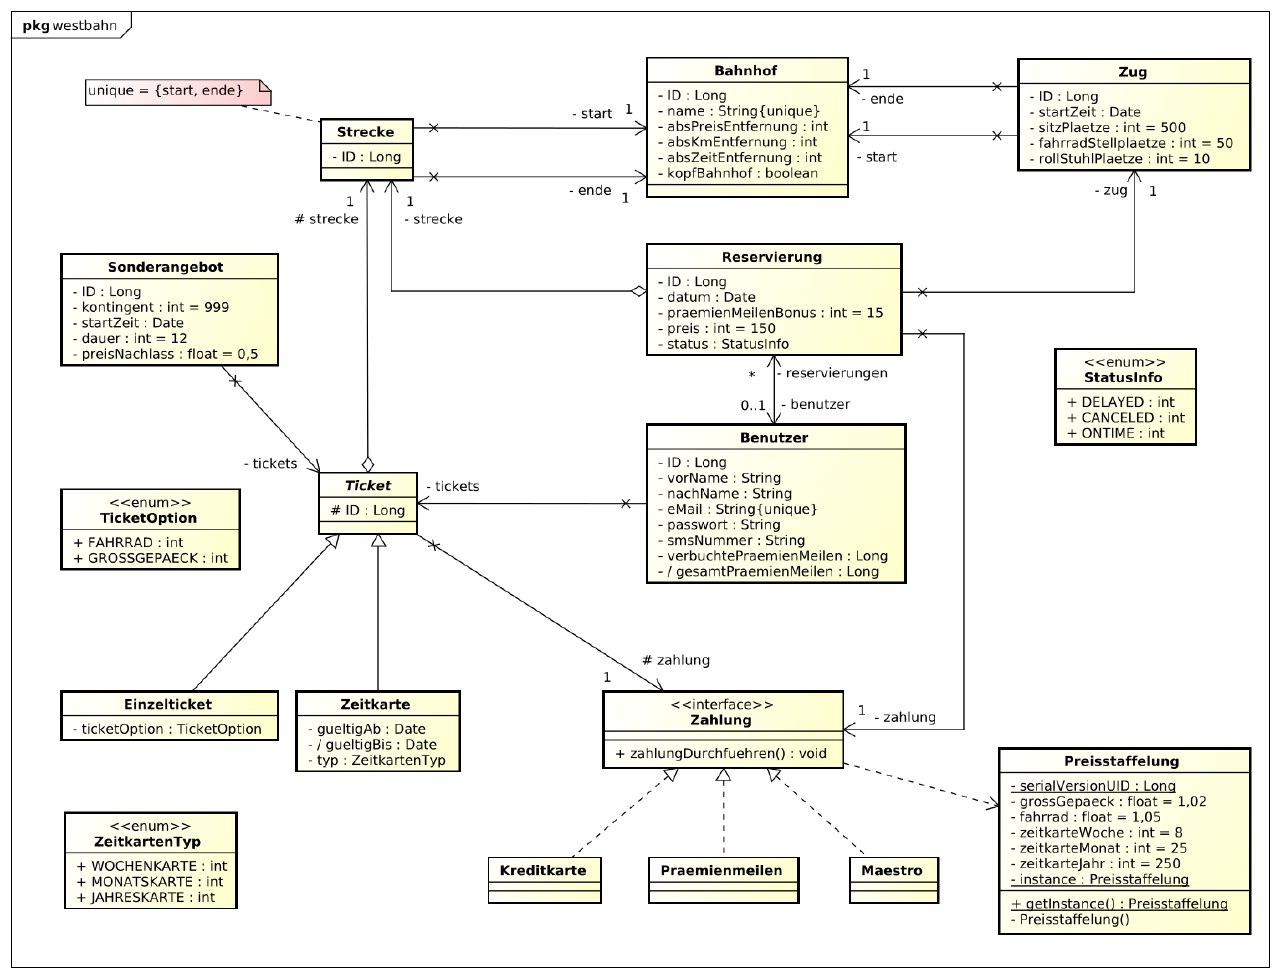
\includegraphics[width=\textwidth]{images/westbahn}
    \caption{Die Westbahn Datenstruktur (UML)}
\end{figure}

\paragraph{Suche}
Die Suche nach Z{\"u}gen muss auf jeden Fall die Auswahl des Abfahrts- und Ankunftsortes (nur folgende Bahnh{\"o}fe sind m{\"o}glich: Wien Westbhf, Wien H{\"u}tteldorf, St. P{\"o}lten, Amstetten, Linz, Wels, Attnang-Puchheim, Salzburg) erm{\"o}glichen. Dies f{\"u}hrt zur Anzeige der m{\"o}glichen Abfahrten, die zur Vereinfachung an jedem Tag zur selben Zeit stattfinden. Des weiteren wird auch die Dauer der Fahrt angezeigt.

In dieser Liste kann nun eine gew{\"u}nschte Abfahrtszeit ausgew{\"a}hlt werden. Die Auswahl der Zeit f{\"u}hrt zu einer automatischen Weiterleitung zum Ticketshop.

Um sich die Auslastung der reservierten Sitzpl{\"a}tze anzusehen, muss bei dem Suchlisting noch das Datum ausgew{\"a}hlt werden. Dieses Service steht jedoch nur registrierten Benutzern zur Verf{\"u}gung.


\paragraph{Ticketshop}
Man kann Einzeltickets kaufen, Reservierungen f{\"u}r bestimmte Z{\"u}ge durchf{\"u}hren und Zeitkarten erwerben. Dabei sind folgende Angaben notwendig:

Einzeltickets: Strecke (Abfahrt/Ankunft), Anzahl der Tickets, Optionen (Fahrrad, Großgep{\"a}ck)
Reservierung: Strecke (Abfahrt/Ankunft), Art der Reservierung (Sitzplatz, Fahrrad, Rollstuhlstellplatz), Reisetag und Zug (Datum/Uhrzeit)
Zeitkarte: Strecke, Zeitraum (Wochen- und Monatskarte)

Um einen {\"U}berblick zu erhalten, kann der Warenkorb beliebig bef{\"u}llt und jederzeit angezeigt werden. Es sind keine {\"a}nderungen erlaubt, jedoch k{\"o}nnen einzelne Posten wieder gel{\"o}scht werden.

Die Funktion „Zur Kassa gehen“ soll die Bezahlung und den Ausdruck der Tickets sowie die Zusendung per eMail/SMS erm{\"o}glichen. Dabei ist f{\"u}r die Bezahlung nur ein Schein-Service zu verwenden um zum Beispiel eine Kreditkarten- bzw. Maestrotransaktion zu simulieren.


\paragraph{Pr{\"a}mienmeilen}
Benutzer k{\"o}nnen sich am System registrieren um get{\"a}tigte K{\"a}ufe und Reservierungen einzusehen. Diese f{\"u}hren n{\"a}mlich zu Pr{\"a}mienmeilen, die weitere Verg{\"u}nstigungen erm{\"o}glichen. Um diese beim n{\"a}chsten Einkauf n{\"u}tzen zu k{\"o}nnen, muss sich der Benutzer einloggen und wird beim „Zur Kassa gehen“ gefragt, ob er die Pr{\"a}mienmeilen f{\"u}r diesen Kauf einl{\"o}sen m{\"o}chte.


Instant Notification System der Warteliste
Der Kunde soll {\"u}ber {\"a}nderungen bez{\"u}glich seiner Reservierung (Versp{\"a}tung bzw. Stornierung) mittels ausgesuchtem Service (eMail bzw. SMS) benachrichtigt werden. Bei ausgelasteten Z{\"u}gen soll auch die M{\"o}glichkeit einer Anfrage an reservierte Pl{\"a}tze m{\"o}glich sein. Dabei kann ein Zuggast um einen Platz ansuchen, bei entsprechender {\"a}nderung einer schon get{\"a}tigten Reservierung wird der ansuchende Kunde informiert und es wird automatisch seine Reservierung angenommen.


\paragraph{Sonderangebote}
F{\"u}r festzulegende Fahrtstrecken soll es erm{\"o}glicht werden, dass ein fixes Kontingent von Tickets (z.b.: 999) zu einem verbilligten Preis (z.b.: 50% Reduktion) angeboten wird. Diese Angebote haben neben dem Kontingent auch eine zeitliche Beschr{\"a}nkung. Der Start wird mit Datum und Uhrzeit festgelegt. Die Dauer wird in Stunden angegeben. Diese Angebote werden automatisch durch Ablauf der Dauer beendet.

\paragraph{Task 1 - Mapping}

Schreiben Sie f{\"u}r alle oben definierten Klassen und Relationen entsprechende Hibernate JPA Implementierungen (javax.persistence.*). Bis auf die Klasse Reservierung sollen daf{\"u}r die Annotationen verwendet werden. Die Klasse Reservierung soll mittels XML Mapping definiert werden.

\paragraph{Task 2 - Named Queries}

Schreiben Sie folgende NamedQueries (kein plain SQL und auch keine Inline-Queries) f{\"u}r das Dom{\"a}nenmodell aus Task1. Die Queries sollen die entsprechenden Parameter akzeptieren und die gew{\"u}nschten Typen zur{\"u}ckliefern:

\begin{enumerate}
    \item Finde alle Reservierungen f{\"u}r einen bestimmten Benutzer, der durch die eMail-Adresse definiert wird.
    \item Liste alle Benutzer auf, die eine Monatskarte besitzen.
    \item Liste alle Tickets f{\"u}r eine bestimmte Strecke aus (durch Anfangs- und Endbahnhof definiert), wo keine Reservierungen durchgef{\"u}hrt wurden.
\end{enumerate}

\paragraph{Task 3 - Validierung}

Alle Constraints der einzelnen Entit{\"a}ten sollen verifiziert werden. Hierf{\"u}r soll die Bean Validation API verwendet werden. Folgende Einschr{\"a}nkungen sollen {\"u}berpr{\"u}ft werden:

\begin{enumerate}
    \item Zug und Strecke k{\"o}nnen nicht denselben Start- und Endbahnhof besitzen.
    \item Die eMail des Benutzers soll ein g{\"a}ngiges eMail-Pattern befolgen.
    \item Die Startzeit eines Sonderangebotes kann nicht in der Vergangenheit liegen.
    \item Der Name eines Bahnhofs darf nicht k{\"u}rzer als zwei und nicht l{\"a}nger als 150 Zeichen sein. Sonderzeichen sind bis auf den Bindestrich zu unterbinden.
\end{enumerate}

\subsection{Bewertung}

\begin{itemize}
    \item Gruppengr{\"o}sse: 1 Person
    \item Anforderungen "{\"u}berwiegend erf{\"u}llt"
    \begin{itemize}
        \item Dokumentation und Beschreibung der angewendeten Schnittstelle
        \item Task 1
        \item Task 2
    \end{itemize}
    \item Anforderungen "zur G{\"a}nze erf{\"u}llt"
    \begin{itemize}
        \item Task 3
        \item Ausreichende Testobjekte zur Validierung der Persistierung
        \item {\"U}berpr{\"u}fung der funktionalen Anforderungen mittels Regressionstests
    \end{itemize}
\end{itemize}

\subsection{Quellen}

''The Java EE Tutorial - Persistence''; Oracle; online: https://docs.oracle.com/javaee/7/tutorial/partpersist.htm\#BNBPY

''HTML5 - A vocabulary and associated APIs for HTML and XHTML''; W3C; 17.12.2012; online: https://www.w3.org/TR/2012/CR-html5-20121217/forms.html\#valid-e-mail-address

''Hibernate ORM Documentation''; JBoss; online: http://hibernate.org/orm/documentation/5.2/l

''Hibernate ORM 5.2.13 Final User Guide''; JBoss; 25.01.2018; online: https://docs.jboss.org/hibernate/orm/5.2/userguide/html\_single/Hibernate\_User\_Guide.html
\clearpage
 	% Information about the purpose of this project
%!TEX root=../main.tex	% Optional

\section{Lösung}

\subsection{Vorbereitung}

Als Projekt wird eine \textbf{Java EE 8} Application mit folgenden Frameworks erstellt:
\begin{itemize}
    \item \textbf{Maven} - Package/Library Management System
    \item \textbf{Java Persistence API} - Annotation Declarations für Entities und das ORM System
    \item \textbf{Hibernate} - Die Implementierung von \gls{jpa}
    \item \textbf{\gls{jdbc}} - Java Datenbank Interface
    \item \textbf{log4j} - Java Logger API
\end{itemize}
\textbf{IntelliJ} lädt automatisch benötigte Libraries, andernfalls kann man dies manuell hinzufügen.

Maven wird bei dem Menüpunkt \textbf{Project Dependencies} ausgewählt.

Mittels Maven können nun alle Libraries hinzugefügt werden:

\begin{itemize}
    \item MySQL:
        \begin{code}{xml}
        <dependency>
            <groupId>mysql</groupId>
            <artifactId>mysql-connector-java</artifactId>
            <version>6.0.6</version>
        </dependency>
        \end{code}
    \item Hibernate (inklusive \gls{jpa}):
        \begin{code}{xml}
        <dependency>
            <groupId>org.hibernate</groupId>
            <artifactId>hibernate-core</artifactId>
            <version>5.2.16.Final</version>
        </dependency>
        \end{code}
    \item log4j:
        \begin{code}{xml}
        <dependency>
            <groupId>log4j</groupId>
            <artifactId>log4j</artifactId>
            <version>1.2.17</version>
        </dependency>
        \end{code}
    \item XML Bind:
        \begin{code}{xml}
        <dependency>
            <groupId>javax.xml.bind</groupId>
            <artifactId>jaxb-api</artifactId>
            <version>2.3.0</version>
        </dependency>
        \end{code}
\end{itemize}

Das \textbf{Maven} \gls{pom} sieht dementsprechend folgendermaßen aus:

\begin{code}{xml}
<!--pom.xml-->
<?xml version="1.0" encoding="UTF-8"?>
<project xmlns="http://maven.apache.org/POM/4.0.0" >
    <modelVersion>4.0.0</modelVersion>

    <groupId>mrousavy</groupId>
    <artifactId>Westbahnhof</artifactId>
    <version>1.0</version>

    <dependencies>
        <dependency>
            <groupId>mysql</groupId>
            <artifactId>mysql-connector-java</artifactId>
            <version>6.0.6</version>
        </dependency>
        <dependency>
            <groupId>org.hibernate</groupId>
            <artifactId>hibernate-core</artifactId>
            <version>5.2.16.Final</version>
        </dependency>
        <dependency>
            <groupId>log4j</groupId>
            <artifactId>log4j</artifactId>
            <version>1.2.17</version>
        </dependency>
        <dependency>
            <groupId>javax.xml.bind</groupId>
            <artifactId>jaxb-api</artifactId>
            <version>2.3.0</version>
        </dependency>
    </dependencies>
</project>
\end{code}

\clearpage
\subsection{Datenbank}

Als Datenbank habe ich mich für eine MySQL 5 Datenbank entschieden, welche in einem Docker \cite{wiki:docker} Container laufen wird.

Dazu habe ich mir eine Dockerfile \cite{docker:dockerfile} geschrieben, welche diesen angepassten MySQL Container zusammenbaut.

Das vollständige Dockerfile schaut dementsprechend folgendermaßen aus:

\begin{code}{Dockerfile}
FROM mysql:latest

ENV MYSQL_ROOT_PASSWORD=root

ENV MYSQL_DATA_DIR=/var/lib/mysql \
    MYSQL_RUN_DIR=/run/mysqld \
    MYSQL_LOG_DIR=/var/log/mysql

ADD ["db_dump.sql", "/tmp/dump.sql"]
COPY ./db_dump.sql /docker-entrypoint-initdb.d/

RUN /etc/init.d/mysql start && mysql -u root -p$\{MYSQL_ROOT_PASSWORD\} < /tmp/dump.sql

EXPOSE 3306
\end{code}

Wobei das \texttt{db\_dump.sql} Create-Script nur die Datenbank erstellt:

\begin{code}{sql}
DROP DATABASE IF EXISTS westbahn;
CREATE DATABASE westbahn;
USE westbahn;
\end{code}

\

Um den Container zu kompilieren verwende ich folgendes script:

\begin{code}{sh}
#!/bin/bash

docker stop mysql
docker rm mysql

docker build -t mysqlimg .
sleep 2
docker run -d --name mysql -v /home/mrousavy/Dockerfiles/data:/var/lib/mysql mysqlimg
\end{code}

Und gestartet kann er mit

\begin{code}{sh}
docker start mysql
\end{code}

werden. In meinem Fall ist die IP Addresse des Containers \texttt{172.17.0.2}.

\clearpage
\subsection{JPA Konfiguration}

Die \gls{jpa} (bzw. Hibernate) muss korrekt konfiguriert werden. Unter anderem muss die SQL Verbindung und der Typ festgelegt werden.

Die Konfigurations-Datei ist eine XML Datei, welche in den App-Resources gespeichert werden muss.

In meinem Fall ist das der relative Pfad: \texttt{src/main/resources/META-INF/persistence.xml}.

Der root tag dieser XML Datei ist ein \texttt{persistence} tag, in welchem die \texttt{persistence-unit} (mit dem \texttt{name} Attribut) definiert wird.

Diese \texttt{persistence-unit} hat verschiedene \texttt{property} tags, welche bestimmte Attribute in der \gls{jpa} konfigurieren.

\

Die vollständige \texttt{persistence.xml} Datei wird folgendermaßen definiert:

\begin{code}{xml}
<?xml version="1.0" encoding="UTF-8"?>
<persistence xmlns="http://java.sun.com/xml/ns/persistence"
                xmlns:xsi="http://www.w3.org/2001/XMLSchema-instance"
                xsi:schemaLocation="http://java.sun.com/xml/ns/persistence http://java.sun.com/xml/ns/persistence/persistence_2_0.xsd"
                version="2.0" >

    <persistence-unit name="westbahn" >
        <description>Westbahn Persistence Configuration XML file</description>
        <provider>org.hibernate.jpa.HibernatePersistenceProvider</provider>

        <properties>
            <!-- MySQL -->
            <property name="hibernate.connection.url" value="jdbc:mysql://172.17.0.2:3306/westbahn" />
            <property name="hibernate.connection.username" value="root" />
            <property name="hibernate.connection.password" value="root" />
            <property name="hibernate.connection.driver" value="com.mysql.jdbc.Driver" />
            <property name="hibernate.dialect" value="org.hibernate.dialect.MySQL5Dialect" />

            <property name="hibernate.hbm2ddl.auto" value="create"/>
            <property name="hibernate.show_sql" value="true"/>
            <property name="hibernate.format_sql" value="true"/>
        </properties>
    </persistence-unit>
</persistence>
\end{code}

\clearpage
\subsection{Entities}

Entities sind einfache Klassen, bzw. \gls{pojo}, welche durch die \gls{jpa} auf die Datenbank \textit{gemapped} \cite{wiki:mapping} werden.

\

Für die Westbahn, müssen alle Entities in dem UML (Siehe: Figur~\ref{fig:uml}) implementiert werden.

Je \gls{entity} muss ein \gls{pojo} erstellt werden, welches eine von der \gls{jpa} verwaltete Schnittstelle zwischen dem Java Code und der Datenbank repräsentiert.

\subsubsection{Astah}

Die Entities habe ich aus dem Astah UML Diagramm exportiert: \textbf{Tool -> Java -> Export Java}

Astah hat nun alle Klassen aus dem UML Diagramm exportiert, welche aber noch alle \gls{jpa} \textbf{Annotations} erhalten werden.

\subsubsection{Java Klassen}

\textbf{Annotations} sind Metadata informationen, welche zur Kompilierung (bei Ausnahmefällen: Auch zur Laufzeit) Klassen, Attributen oder Methoden hinzugefügt werden können.

Die wichtigste \textbf{Annotation} ist:
\begin{code}{java}
@Entity
public class Bahnhof {}
\end{code}

welche auf jedem \textit{gemappten} \cite{wiki:mapping} \gls{pojo} zu finden ist.

\

Außerdem sollte jede Entity eine eindeutige Identifikation haben, oft durch eine Ganzzahl mit dem namen \texttt{ID}.

Beispielsweise könnte so die ID von einem Bahnhof ausschauen:

\begin{code}{java}
@Id
@GeneratedValue(strategy = GenerationType.IDENTITY)
private long ID;
\end{code}

wobei die \textbf{Annotation} \texttt{@GeneratedValue} der \gls{jpa} mitteilt, es handelt sich um ein generiertes Attribut welches im Idealfall nicht vom Benutzer modifiziert wird. Beispielsweise wäre dies eine automatisch mitzählende Identifikation.

\

Alle anderen Attribute bzw. \textbf{Properties} können zusätzliche \textbf{Annotations} erhalten, sind jedoch optional. Beispielsweise kann ein name auch einzigartig sein:

\begin{code}{java}
@Column(unique = true)
private String name;
\end{code}

\

Mit etwas \gls{ide} Zauberei können auch getter und setter Methoden generiert werden, womit das \gls{pojo} - und nun auch die \gls{entity} - nun so ausschaut:

\begin{code}{java}
package BusinessObjects;

import javax.persistence.*;
import java.io.Serializable;

@Entity
public class Bahnhof {
	@Id
	@GeneratedValue(strategy = GenerationType.IDENTITY)
	private long ID;

	@Column(unique = true)
	private String name;

	private int absPreisEntfernung;

	private int absKmEntfernung;

	private int absZeitEntfernung;

	private boolean kopfBahnhof;

    public long getID() {
        return ID;
    }

    public void setID(long ID) {
        this.ID = ID;
    }

    public String getName() {
        return name;
    }

    public void setName(String name) {
        this.name = name;
    }

    public int getAbsPreisEntfernung() {
        return absPreisEntfernung;
    }

    public void setAbsPreisEntfernung(int absPreisEntfernung) {
        this.absPreisEntfernung = absPreisEntfernung;
    }

    public int getAbsKmEntfernung() {
        return absKmEntfernung;
    }

    public void setAbsKmEntfernung(int absKmEntfernung) {
        this.absKmEntfernung = absKmEntfernung;
    }

    public int getAbsZeitEntfernung() {
        return absZeitEntfernung;
    }

    public void setAbsZeitEntfernung(int absZeitEntfernung) {
        this.absZeitEntfernung = absZeitEntfernung;
    }

    public boolean isKopfBahnhof() {
        return kopfBahnhof;
    }

    public void setKopfBahnhof(boolean kopfBahnhof) {
        this.kopfBahnhof = kopfBahnhof;
    }
}
\end{code}

\

Dementsprechend müssen nun alle \gls{pojo}s zu \textbf{Entities} gemacht werden.

\

Ein Sonderfall war die \gls{entity} Strecke (\texttt{Strecke.java}), da diese \textit{unique constraints} benötigte.

Dazu gefunden habe ich die Dokumentation in den Java Docs: \gls{uniqueConstraints}, welche zu folgendem Code für die \gls{entity} \textbf{Strecke} führte:

\begin{code}{java}
@Table(
        uniqueConstraints = @UniqueConstraint(columnNames = {"start_id", "ende_id"})
)
\end{code}

Die Spalten heißen \texttt{start\_id}/\texttt{end\_id}, da es sich nicht um Scalar-Properties, welche standardisierte Datentypen sind, sondern um Navigation-Properties, welche im Hintergrund von der \gls{jpa} zu Foreign Keys verarbeitet werden, hält.

Es wird also kein tatsächliches Bahnhof Objekt auf der Datenbank gespeichert (da dies nicht möglich ist), sondern nur der Foreign Key zu einem Eintrag in dem Bahnhof Table. (Siehe: Mapping \cite{wiki:mapping})

\

Außerdem soll die \texttt{Reservierung} Klasse nicht mittels der \texttt{@Entity} Annotation, sonder mittels \texttt{XML Mapping} \textit{gemapped} werden.

Dazu wird die Ressource \texttt{orm.xml} in dem relativen Ordner \texttt{src/main/resources/META-INF/} erstellt:

\begin{code}{xml}
<?xml version="1.0" encoding="UTF-8" ?>

<entity-mappings xmlns="http://java.sun.com/xml/ns/persistence/orm"
                    xmlns:xsi="http://www.w3.org/2001/XMLSchema-instance"
                    xsi:schemaLocation="http://java.sun.com/xml/ns/persistence/orm
    http://java.sun.com/xml/ns/persistence/orm_1_0.xsd"
                    version="1.0">

    <description>XML Mapping file (ORM)</description>
    <package>BusinessObjects</package>

    <entity class="BusinessObjects.Reservierung" name="Reservierung">
        <table name="Reservierung"/>
        <named-query name="Reservierung.getReservierungenForUser">
            <query>SELECT r FROM Benutzer.reservierungen r INNER JOIN Reservierung ON r.ID=Reservierung.ID WHERE Benutzer.eMail = :email</query>
        </named-query>
        <attributes>
            <id name="ID">
                <generated-value strategy="IDENTITY"/>
            </id>
            <basic name="datum"/>
            <basic name="praemienMeilenBonus"/>
            <basic name="preis"/>
            <basic name="status"/>
            <one-to-one name="zug">
                <join-column name="ID"/>
            </one-to-one>
            <one-to-one name="strecke">
                <join-column name="ID"/>
            </one-to-one>
            <one-to-one name="benutzer">
                <join-column name="ID"/>
            </one-to-one>
            <transient name="zahlung"/>
        </attributes>
    </entity>

</entity-mappings>
\end{code}

\clearpage
\subsection{EntityManager}

\subsubsection{Erstellen}

Sobald alle Entities erstellt wurden, kann man die \texttt{EntityManagerFactory} \cite{jdoc:entityManagerFactory} verwenden um eine Verbindung zur Datenbank aufzubauen und den \texttt{EntityManager} \cite{jdoc:entityManager} erstellen, um mit den \gls{jpa} \textit{gemappten} Entities arbeiten.

\begin{code}{java}
EntityManagerFactory emfactory = Persistence.createEntityManagerFactory("westbahn");
EntityManager entitymanager = emfactory.createEntityManager();
// ...
entitymanager.close();
emfactory.close();
\end{code}

\subsubsection{Create}

Entities können erstellt werden, indem das \gls{pojo} mittels \texttt{new} erstellt wird, und dem \texttt{EntityManager} \textit{angehängt} wird:

\begin{code}{java}
entityManager.getTransaction().begin();
Bahnhof bahnhof = new Bahnhof();
bahnhof.setName("Wien Spittelau");
entitymanager.persist(bahnhof);
entityManager.getTransaction().commit();
\end{code}

Mittels \texttt{persist} wird diese Entity dem \texttt{PersistenceContext} hinzugefügt, es besteht jedoch auch die Möglichkeit die Entity mittels \texttt{merge} hinzuzufügen. Allerdings wird bei \texttt{merge} eine neue Entity mit kopierten Werten erstellt, was ein unnötiger Overhead ist.

\subsubsection{Update}

Um bestimmte Werte einer Entity zu ändern, muss dies an einer Entity welche bereits im \texttt{PersistenceContext} registriert ist getan werden.

Falls diese Entity nur lokal existiert, muss diese zuerst mittels ID über den \texttt{EntityManager} gefunden werden. Es ist wichtig, dass die \textbf{ID} beim aufrufen von \texttt{find} der richtige Datentyp von der Entity ist. (\texttt{long} oder \texttt{int})

\begin{code}{java}
entityManager.getTransaction().begin();
Bahnhof bahnhof = entityManager.find(Bahnhof.class, BAHNHOF_ID);
bahnhof.setName("Wien Heiligenstadt");
entityManager.flush();
entityManager.getTransaction().commit();
\end{code}

\subsubsection{Remove}

Um eine Entity zu entfernen muss sie zuerst gefunden werden (oder bereits im \texttt{PersistenceContext} vorhanden sein) und dann mittels \texttt{remove} entfernt werden:

\begin{code}{java}
entityManager.getTransaction().begin();
Bahnhof bahnhof = entityManager.find(Bahnhof.class, BAHNHOF_ID);
entityManager.remove(bahnhof);
entityManager.flush();
entityManager.getTransaction().commit();
\end{code}

\clearpage
\subsection{Named Queries}

\textbf{Finde alle Reservierungen für einen bestimmten Benutzer, der durch die eMail-Adresse definiert wird.}

\begin{code}{java}
@NamedQuery(
    name="Reservierung.getReservierungenForUser",
    query = "SELECT r FROM Benutzer.reservierungen r INNER JOIN Reservierung ON r.ID=Reservierung.ID WHERE Benutzer.eMail = :email"
)
\end{code}

\textbf{Liste alle Benutzer auf, die eine Monatskarte besitzen.}

Hierbei war die Schwierigkeit die richtigen \texttt{JOIN}s zu finden, da die \texttt{Benutzer.tickets} Liste in Wirklichkeit von \textbf{Hibernate} aus dem versteckten Table \texttt{Benutzer\_Tickets} verlinkt wird. Also muss irgendwie Zugriff auf die \texttt{Benutzer.tickets} Liste, den \texttt{Benutzer} selbst \textbf{und} den \texttt{Ticket.typ} gewährt werden.

\begin{code}{java}
@NamedQuery(
    name = "Benutzer.getAllWithMonatskarte",
    query = "SELECT Benutzer FROM Benutzer.tickets t INNER JOIN Zeitkarte ON Zeitkarte.ID=t.ID WHERE Zeitkarte.typ=1"
)
\end{code}

\textbf{Liste alle Tickets für eine bestimmte Strecke aus (durch Anfangs- und Endbahnhof definiert), wo keine Reservierungen durchgeführt wurden.}

\begin{code}{java}
// ...
\end{code}

\clearpage
\subsection{Constraints}

Es soll die \textbf{Bean Validation API} verwendet werden, um bestimmte Attribute einzugrenzen.

Als Referenz habe ich den Bean Validation Cheat Sheet von owasp \cite{owasp:beanValidationCheatSheet} verwendet.

\subsubsection{Unique}
\textbf{Zug und Strecke können nicht denselben Start- und Endbahnhof besitzen.}

Gelöst habe ich dies mittels der \texttt{@AssertTrue} Annotation:

\begin{code}{java}
@AssertTrue(message="Start und End Bahnhof können nicht die selben sein!")
public boolean validBahnhof() {
    return !start.equals(ende);
}
\end{code}

\subsubsection{eMail}
\textbf{Die eMail des Benutzers soll ein gängiges eMail-Pattern befolgen.}

Gelöst habe ich dies mittels der \texttt{@Email} Annotation:

\begin{code}{java}
@Email
private String eMail;

public void seteMail(@Email String eMail) {
    this.eMail = eMail;
}
\end{code}

\subsubsection{Startzeit}
\textbf{Die Startzeit eines Sonderangebotes kann nicht in der Vergangenheit liegen.}

Gelöst habe ich dies mittels der \texttt{@Future} Annotation:

\begin{code}{java}
@Future
private Date startZeit;

public void setStartZeit(@Future Date startZeit) {
    this.startZeit = startZeit;
}
\end{code}

\subsubsection{Bahnhofname}
\textbf{Der Name eines Bahnhofs darf nicht kürzer als zwei und nicht länger als 150 Zeichen sein. Sonderzeichen sind bis auf den Bindestrich zu unterbinden.}

Gelöst habe ich dies mittels den \texttt{@Size} und \texttt{@Pattern} Annotations:
\begin{code}{java}
@Column(unique = true)
@Size(min=2, max=150)
@Pattern(regexp = "^[a-zA-Z0-9\\-]$")
private String name;
\end{code}

\clearpage
\subsection{Testen}

\subsubsection{Logger}

Dadurch dass wir einen Logger (mittels \textbf{log4j}) erstellt haben, wird \gls{jpa} (bzw. Hibernate) auf den Output des Loggers loggen. Mit der Einstellung in der \texttt{persistence.xml} werden auch erstellte Queries geloggt.

Der Logger wurde folgendermaßen konfiguriert und erstellt:

\begin{code}{properties}
# Root logger option
log4j.rootLogger=INFO, console

log4j.logger.com.javarticles=INFO, console
log4j.logger.com.javarticles.log4j=INFO, console
log4j.logger.com.javarticles.log4j.info.Log4jInfoExample=INFO, console
log4j.logger.com.javarticles.log4j.warn.Log4jWarnExample=WARN, console

# Direct log messages to stdout
log4j.appender.console=org.apache.log4j.ConsoleAppender
log4j.appender.console.Target=System.out
log4j.appender.console.layout=org.apache.log4j.PatternLayout
log4j.appender.console.layout.ConversionPattern=%d{HH:mm}| %p | %F %L | %m%n
\end{code}

In Java:

\begin{code}{java}
private static final Logger _logger = LogManager.getLogger(Main.class.getName());
\end{code}

\subsubsection{Test Programm}

Das Test Programm (\texttt{Main.java}) habe ich geschrieben, um das erstellen, modifizieren und entfernen von einem Bahnhof zu testen.

\begin{code}{java}
import BusinessObjects.Bahnhof;
import org.apache.log4j.LogManager;
import org.apache.log4j.Logger;

import javax.persistence.EntityManager;
import javax.persistence.EntityManagerFactory;
import javax.persistence.Persistence;

public class Main {
    private static final Logger logger = LogManager.getLogger(Main.class.getName());
    private static final long BAHNHOF_ID = 1L;

    public static void main(String[] args) {
        logger.info("Starting EntityManagerFactory..");
        EntityManagerFactory factory = Persistence.createEntityManagerFactory("westbahn");
        EntityManager entityManager = factory.createEntityManager();

        create(entityManager);
        update(entityManager);
        remove(entityManager);

        entityManager.close();
        factory.close();
        logger.info("Finished!");
    }

    private static void create(EntityManager entityManager) {
        logger.info("Creating Bahnhof Spittelau..");
        entityManager.getTransaction().begin();
        Bahnhof bahnhof = new Bahnhof();
        bahnhof.setName("Wien Spittelau");
        entityManager.persist(bahnhof);
        entityManager.getTransaction().commit();
        logger.info("Bahnhof Spittelau created!");
    }

    private static void update(EntityManager entityManager) {
        logger.info("Updating Bahnhof Spittelau -> Heiligenstadt..");
        entityManager.getTransaction().begin();
        Bahnhof bahnhof = entityManager.find(Bahnhof.class, BAHNHOF_ID);
        bahnhof.setName("Wien Heiligenstadt");
        entityManager.flush();
        entityManager.getTransaction().commit();
        logger.info("Bahnhof Spittelau updated to Heiligenstadt!");
    }

    private static void remove(EntityManager entityManager) {
        logger.info("Removing Bahnhof Heiligenstadt..");
        entityManager.getTransaction().begin();
        Bahnhof bahnhof = entityManager.find(Bahnhof.class, BAHNHOF_ID);
        entityManager.remove(bahnhof);
        entityManager.flush();
        entityManager.getTransaction().commit();
        logger.info("Bahnhof Heiligenstadt removed!");
    }
}
\end{code}

Output:

\begin{code}{text}
13:58| INFO | Main.java 29 | Creating Bahnhof Spittelau..
Hibernate:
    insert
    into
        Bahnhof
        (absKmEntfernung, absPreisEntfernung, absZeitEntfernung, kopfBahnhof, name)
    values
        (?, ?, ?, ?, ?)
13:58| INFO | Main.java 35 | Bahnhof Spittelau created!
13:58| INFO | Main.java 39 | Updating Bahnhof Spittelau -> Heiligenstadt..
Hibernate:
    update
        Bahnhof
    set
        absKmEntfernung=?,
        absPreisEntfernung=?,
        absZeitEntfernung=?,
        kopfBahnhof=?,
        name=?
    where
        ID=?
13:58| INFO | Main.java 45 | Bahnhof Spittelau updated to Heiligenstadt!
13:58| INFO | Main.java 49 | Removing Bahnhof Heiligenstadt..
Hibernate:
    delete
    from
        Bahnhof
    where
        ID=?
13:58| INFO | Main.java 55 | Bahnhof Heiligenstadt removed!
13:58| INFO | DriverManagerConnectionProviderImpl.java 233 | HHH10001008: Cleaning up connection pool [jdbc:mysql://172.17.0.2:3306/westbahn]
13:58| INFO | Main.java 25 | Finished!
\end{code}

 % Solution for the given tasks and their documentation
% \glsaddall 		% Add all glossary entries to printglossaries
\end{document}
